\chapter{Analyse}
Ein erster Prototyp konnte gemäss Kapitel \ref{chapter:Realisierung} (Realisierung) Ende Mai 2020 umgesetzt werden.
Während einer vierwöchigen Testphase konnten so anschliessend im laufenden Betrieb Statistikdaten zur Benutzung gesammelt werden.
Die Sammlung besteht nur aus Informationen zu den Uploads (=Nutzung der Hochladelinks).
Bei den Downloadlinks ist eine Auswertung nicht aussagekräftig, da über den Browser keine Informationen gesammelt werden können, wann ein Download fertig ist. 
Aus Sicht des Synology NAS wird die Datei als ganzes angeboten. Der Kunde kann aber Downloads pausieren oder gar durch ein Download-Tools ausführen anstelle eines Browsers.

\section{Aggregierte Logfiles}
Total wurden 94 Dateiübertragungen vorgenommen. Bei den 94 Übertragungen sind 253 Dateien übermittelt worden.
Von der kleinsten Datei mit 11Kb bis hin zu Grössten mit 10GB wurde der Prototyp für ein breites Spektrum genutzt.
Die grossen Dateien wurden in Total 1193 Teile zerlegt und am Ende der Übermittelung wieder zusammengesetzt. 
Die Summe aller Dateieigrössen entspricht ca. 70GB welche innert 120 Minuten übertragen wurden. 
Auf den ersten Blick mag dies nicht sonderlich ideal wirken, darauf wird daher im nächsten Abschnitt genauer eingegangen.

\section{Performanz aus Logfiles}
Eine reguläre Durchschnittsrechnung ist wenig sinnvoll bei den gesammelten Daten. 
Der Grössenunterschied der Dateien ist dafür zu gross. Es wurden Verhältnismässig viele kleinere Dateien übertragen und wenige grosse,
wie in Abbildung \ref{fig:diagramme2} ersichtlich.

\begin{figure}[!h]
    \centering
    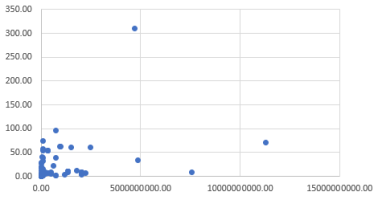
\includegraphics[width=0.5\linewidth]{content/images/diagramme2.png}
    \caption{Verhältnis Dateigrösse (x) zu Geschwindigkeit (y)}
    \label{fig:diagramme2}
\end{figure} 


Zur sinnvollen Beurteilung werden daher Boxplots gebildet um die Verteilung zu bestimmen und auf den Median einzugehen.
\begin{figure}[!h]
    \centering
    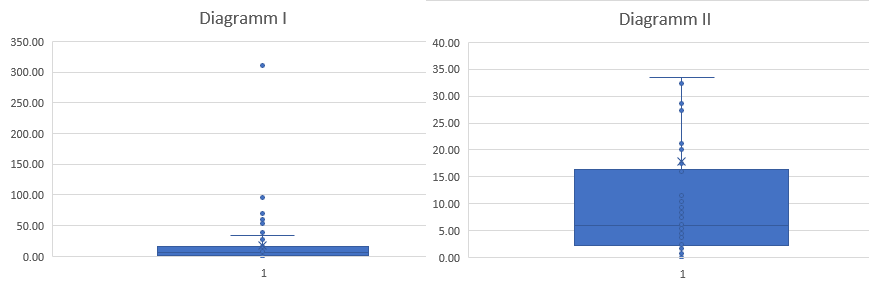
\includegraphics[width=1\linewidth]{content/images/diagramme.png}
    \caption{Boxplot der Geschwindigkeiten}
    \label{fig:diagramme}
\end{figure} 

Die vielen Ausreisser im ersten Teil der Grafik \ref{fig:diagramme} lassen sich durch die Internet-Geschwindigkeit der Benutzer erklären.
Innerhalb der Schweiz werden sowohl Kupfer als auch Glasfaseranschlüsse verwendet.
Die gesammelten Daten reichen nicht aus, um hier eine Kategorisierung oder Aufteilung nach Anschlussart zu ermöglichen.
Die Vermutung liegt jedoch nahe, dass die Ausreisse nach oben durch wenige Übermittlungen mit Glasfaseranschlüssen verursacht werden.
Zur besseren Lesbarkeit ist der zweite Teil der Grafik ohne die Ausreisse aufgebaut. 
Die mediane Wartezeit für den Upload liegt bei nur 7.85 Sekunden. Eine kurzweilige Zeitspanne, die sich als Benutzer beim Hochladen gut abwarten lässt.
Die mediane Geschwindigkeit von 5.88 MB/S wirkt langsam, ist es aber keineswegs. 
Es entspricht ungefähr der von Salt \cite{Salt} publizierten schweizweiten mittleren Upload-Geschwindigkeit. Die genannten 55 MBit/s entsprechen ca. 6.8 MB/S.

Die keine Differenz lässt sich nebst der Anschluss-Technologie auch durch das Teilen und Zusammensetzen der grossen Dateien erklären.
Das Log hat die Zeit dafür ebenfalls beim Hochladen mitgezählt. 


\section{Fazit}
Im Laufe dieser Arbeit konnte der konzeptionierte Prototyp erfolgreich implementiert werden.
Der Prototyp wurde innerhalb der Testphase überraschende 94 mal verwendet. Das entspricht mehreren Nutzungen pro Arbeitstag.
Die häufige Verwendung lässt darauf schliessen, dass der Prototyp sehr guten Anklang findet.
Folglich kann von einer einfachen, selbstsprechenden Nutzung ausgegangen werden. 
Ganz so, wie es bei der Spezifikation gewünscht wurde. Die erzielte Performanz ist gut annehmbar. 
Der Prototyp hat durchaus noch einiges an Verbesserungspotential, vor allem beim Umgang mit den grossen Dateien.
Während der Testphase sind keinerlei negative Rückmeldungen eingegangen. 
Dies spricht mit den anderen Resultaten dafür, die Richtung beizubehalten und eine Weiterentwicklung am Prototyp zu verfolgen.